\documentclass[]{article}
\usepackage{lmodern}
\usepackage{amssymb,amsmath}
\usepackage{ifxetex,ifluatex}
\usepackage{fixltx2e} % provides \textsubscript
\ifnum 0\ifxetex 1\fi\ifluatex 1\fi=0 % if pdftex
  \usepackage[T1]{fontenc}
  \usepackage[utf8]{inputenc}
\else % if luatex or xelatex
  \ifxetex
    \usepackage{mathspec}
  \else
    \usepackage{fontspec}
  \fi
  \defaultfontfeatures{Ligatures=TeX,Scale=MatchLowercase}
\fi
% use upquote if available, for straight quotes in verbatim environments
\IfFileExists{upquote.sty}{\usepackage{upquote}}{}
% use microtype if available
\IfFileExists{microtype.sty}{%
\usepackage{microtype}
\UseMicrotypeSet[protrusion]{basicmath} % disable protrusion for tt fonts
}{}
\usepackage[margin=1in]{geometry}
\usepackage{hyperref}
\hypersetup{unicode=true,
            pdftitle={Reproducible Research: Peer Assessment 1},
            pdfauthor={Abdul Rasheed Narejo},
            pdfborder={0 0 0},
            breaklinks=true}
\urlstyle{same}  % don't use monospace font for urls
\usepackage{color}
\usepackage{fancyvrb}
\newcommand{\VerbBar}{|}
\newcommand{\VERB}{\Verb[commandchars=\\\{\}]}
\DefineVerbatimEnvironment{Highlighting}{Verbatim}{commandchars=\\\{\}}
% Add ',fontsize=\small' for more characters per line
\usepackage{framed}
\definecolor{shadecolor}{RGB}{248,248,248}
\newenvironment{Shaded}{\begin{snugshade}}{\end{snugshade}}
\newcommand{\AlertTok}[1]{\textcolor[rgb]{0.94,0.16,0.16}{#1}}
\newcommand{\AnnotationTok}[1]{\textcolor[rgb]{0.56,0.35,0.01}{\textbf{\textit{#1}}}}
\newcommand{\AttributeTok}[1]{\textcolor[rgb]{0.77,0.63,0.00}{#1}}
\newcommand{\BaseNTok}[1]{\textcolor[rgb]{0.00,0.00,0.81}{#1}}
\newcommand{\BuiltInTok}[1]{#1}
\newcommand{\CharTok}[1]{\textcolor[rgb]{0.31,0.60,0.02}{#1}}
\newcommand{\CommentTok}[1]{\textcolor[rgb]{0.56,0.35,0.01}{\textit{#1}}}
\newcommand{\CommentVarTok}[1]{\textcolor[rgb]{0.56,0.35,0.01}{\textbf{\textit{#1}}}}
\newcommand{\ConstantTok}[1]{\textcolor[rgb]{0.00,0.00,0.00}{#1}}
\newcommand{\ControlFlowTok}[1]{\textcolor[rgb]{0.13,0.29,0.53}{\textbf{#1}}}
\newcommand{\DataTypeTok}[1]{\textcolor[rgb]{0.13,0.29,0.53}{#1}}
\newcommand{\DecValTok}[1]{\textcolor[rgb]{0.00,0.00,0.81}{#1}}
\newcommand{\DocumentationTok}[1]{\textcolor[rgb]{0.56,0.35,0.01}{\textbf{\textit{#1}}}}
\newcommand{\ErrorTok}[1]{\textcolor[rgb]{0.64,0.00,0.00}{\textbf{#1}}}
\newcommand{\ExtensionTok}[1]{#1}
\newcommand{\FloatTok}[1]{\textcolor[rgb]{0.00,0.00,0.81}{#1}}
\newcommand{\FunctionTok}[1]{\textcolor[rgb]{0.00,0.00,0.00}{#1}}
\newcommand{\ImportTok}[1]{#1}
\newcommand{\InformationTok}[1]{\textcolor[rgb]{0.56,0.35,0.01}{\textbf{\textit{#1}}}}
\newcommand{\KeywordTok}[1]{\textcolor[rgb]{0.13,0.29,0.53}{\textbf{#1}}}
\newcommand{\NormalTok}[1]{#1}
\newcommand{\OperatorTok}[1]{\textcolor[rgb]{0.81,0.36,0.00}{\textbf{#1}}}
\newcommand{\OtherTok}[1]{\textcolor[rgb]{0.56,0.35,0.01}{#1}}
\newcommand{\PreprocessorTok}[1]{\textcolor[rgb]{0.56,0.35,0.01}{\textit{#1}}}
\newcommand{\RegionMarkerTok}[1]{#1}
\newcommand{\SpecialCharTok}[1]{\textcolor[rgb]{0.00,0.00,0.00}{#1}}
\newcommand{\SpecialStringTok}[1]{\textcolor[rgb]{0.31,0.60,0.02}{#1}}
\newcommand{\StringTok}[1]{\textcolor[rgb]{0.31,0.60,0.02}{#1}}
\newcommand{\VariableTok}[1]{\textcolor[rgb]{0.00,0.00,0.00}{#1}}
\newcommand{\VerbatimStringTok}[1]{\textcolor[rgb]{0.31,0.60,0.02}{#1}}
\newcommand{\WarningTok}[1]{\textcolor[rgb]{0.56,0.35,0.01}{\textbf{\textit{#1}}}}
\usepackage{graphicx,grffile}
\makeatletter
\def\maxwidth{\ifdim\Gin@nat@width>\linewidth\linewidth\else\Gin@nat@width\fi}
\def\maxheight{\ifdim\Gin@nat@height>\textheight\textheight\else\Gin@nat@height\fi}
\makeatother
% Scale images if necessary, so that they will not overflow the page
% margins by default, and it is still possible to overwrite the defaults
% using explicit options in \includegraphics[width, height, ...]{}
\setkeys{Gin}{width=\maxwidth,height=\maxheight,keepaspectratio}
\IfFileExists{parskip.sty}{%
\usepackage{parskip}
}{% else
\setlength{\parindent}{0pt}
\setlength{\parskip}{6pt plus 2pt minus 1pt}
}
\setlength{\emergencystretch}{3em}  % prevent overfull lines
\providecommand{\tightlist}{%
  \setlength{\itemsep}{0pt}\setlength{\parskip}{0pt}}
\setcounter{secnumdepth}{0}
% Redefines (sub)paragraphs to behave more like sections
\ifx\paragraph\undefined\else
\let\oldparagraph\paragraph
\renewcommand{\paragraph}[1]{\oldparagraph{#1}\mbox{}}
\fi
\ifx\subparagraph\undefined\else
\let\oldsubparagraph\subparagraph
\renewcommand{\subparagraph}[1]{\oldsubparagraph{#1}\mbox{}}
\fi

%%% Use protect on footnotes to avoid problems with footnotes in titles
\let\rmarkdownfootnote\footnote%
\def\footnote{\protect\rmarkdownfootnote}

%%% Change title format to be more compact
\usepackage{titling}

% Create subtitle command for use in maketitle
\newcommand{\subtitle}[1]{
  \posttitle{
    \begin{center}\large#1\end{center}
    }
}

\setlength{\droptitle}{-2em}

  \title{Reproducible Research: Peer Assessment 1}
    \pretitle{\vspace{\droptitle}\centering\huge}
  \posttitle{\par}
    \author{Abdul Rasheed Narejo}
    \preauthor{\centering\large\emph}
  \postauthor{\par}
      \predate{\centering\large\emph}
  \postdate{\par}
    \date{August 27, 2018}


\begin{document}
\maketitle

\hypertarget{introduction}{%
\subsection{Introduction}\label{introduction}}

It is now possible to collect a large amount of data about personal
movement using activity monitoring devices such as a Fitbit,
\href{http://www.fitbit.com/}{Nike}
\href{http://www.nike.com/us/en_us/c/nikeplus-fuelband}{Fuelband}, or
\href{https://jawbone.com/up}{Jawbone Up}. These type of devices are
part of the ``quantified self'' movement -- a group of enthusiasts who
take measurements about themselves regularly to improve their health, to
find patterns in their behavior, or because they are tech geeks. But
these data remain under-utilized both because the raw data are hard to
obtain and there is a lack of statistical methods and software for
processing and interpreting the data.

This assignment makes use of data from a personal activity monitoring
device. This device collects data at 5 minute intervals through out the
day. The data consists of two months of data from an anonymous
individual collected during the months of October and November, 2012 and
include the number of steps taken in 5 minute intervals each day.

The data for this assignment can be downloaded from the course web site:

Dataset:
\href{https://d396qusza40orc.cloudfront.net/repdata\%2Fdata\%2Factivity.zip}{Activity
monitoring data} {[}52K{]} The variables included in this dataset are:

\begin{itemize}
\tightlist
\item
  \textbf{steps}: Number of steps taking in a 5-minute interval (missing
  values are coded as NA)
\item
  \textbf{date}: The date on which the measurement was taken in
  YYYY-MM-DD format
\item
  \textbf{interval}: Identifier for the 5-minute interval in which
  measurement was taken
\end{itemize}

The dataset is stored in a comma-separated-value (CSV) file and there
are a total of 17,568 observations in this dataset.

\hypertarget{load-required-libraries}{%
\subsection{Load required libraries}\label{load-required-libraries}}

\begin{Shaded}
\begin{Highlighting}[]
\KeywordTok{library}\NormalTok{(dplyr) }\CommentTok{# load dplyr for data manipulation}
\KeywordTok{library}\NormalTok{(lattice) }\CommentTok{# lattice for data visualization}
\KeywordTok{library}\NormalTok{(ggplot2) }\CommentTok{# ggplot for data visualization}
\end{Highlighting}
\end{Shaded}

\hypertarget{loading-and-preprocessing-the-data}{%
\subsection{Loading and preprocessing the
data}\label{loading-and-preprocessing-the-data}}

\hypertarget{load-the-data-read.csv}{%
\subsubsection{Load the data
(read.csv())}\label{load-the-data-read.csv}}

\begin{Shaded}
\begin{Highlighting}[]
\NormalTok{data <-}\StringTok{ }\KeywordTok{read.csv}\NormalTok{(}\StringTok{"activity.csv"}\NormalTok{)}
\KeywordTok{summary}\NormalTok{(data}\OperatorTok{$}\NormalTok{steps)}
\end{Highlighting}
\end{Shaded}

\begin{verbatim}
##    Min. 1st Qu.  Median    Mean 3rd Qu.    Max.    NA's 
##    0.00    0.00    0.00   37.38   12.00  806.00    2304
\end{verbatim}

\hypertarget{processtransform-the-data-if-necessary-into-a-format-suitable-for-your-analysis}{%
\subsubsection{Process/transform the data (if necessary) into a format
suitable for your
analysis,}\label{processtransform-the-data-if-necessary-into-a-format-suitable-for-your-analysis}}

\begin{Shaded}
\begin{Highlighting}[]
\CommentTok{# format date column as valid Date format}
\NormalTok{data}\OperatorTok{$}\NormalTok{date <-}\StringTok{ }\KeywordTok{as.Date}\NormalTok{(data}\OperatorTok{$}\NormalTok{date)}

\CommentTok{# generate data summary}
\KeywordTok{summary}\NormalTok{(data)}
\end{Highlighting}
\end{Shaded}

\begin{verbatim}
##      steps             date               interval     
##  Min.   :  0.00   Min.   :2012-10-01   Min.   :   0.0  
##  1st Qu.:  0.00   1st Qu.:2012-10-16   1st Qu.: 588.8  
##  Median :  0.00   Median :2012-10-31   Median :1177.5  
##  Mean   : 37.38   Mean   :2012-10-31   Mean   :1177.5  
##  3rd Qu.: 12.00   3rd Qu.:2012-11-15   3rd Qu.:1766.2  
##  Max.   :806.00   Max.   :2012-11-30   Max.   :2355.0  
##  NA's   :2304
\end{verbatim}

\hypertarget{what-is-mean-total-number-of-steps-taken-per-day}{%
\subsection{What is mean total number of steps taken per
day?}\label{what-is-mean-total-number-of-steps-taken-per-day}}

For this part of the assignment, you can ignore the missing values in
the dataset.

\hypertarget{calculate-the-total-number-of-steps-taken-per-day}{%
\subsubsection{Calculate the total number of steps taken per
day}\label{calculate-the-total-number-of-steps-taken-per-day}}

\begin{Shaded}
\begin{Highlighting}[]
\CommentTok{# calculate total steps by each day}
\NormalTok{dailySteps <-}\StringTok{ }\NormalTok{data }\OperatorTok\StringTok{ }\KeywordTok{group_by}\NormalTok{(date) }\OperatorTok\StringTok{ }\KeywordTok{summarize}\NormalTok{(}\DataTypeTok{dailySteps=}\KeywordTok{sum}\NormalTok{(steps))}
\KeywordTok{summary}\NormalTok{(dailySteps)}
\end{Highlighting}
\end{Shaded}

\begin{verbatim}
##       date              dailySteps   
##  Min.   :2012-10-01   Min.   :   41  
##  1st Qu.:2012-10-16   1st Qu.: 8841  
##  Median :2012-10-31   Median :10765  
##  Mean   :2012-10-31   Mean   :10766  
##  3rd Qu.:2012-11-15   3rd Qu.:13294  
##  Max.   :2012-11-30   Max.   :21194  
##                       NA's   :8
\end{verbatim}

\hypertarget{make-a-histogram-of-the-total-number-of-steps-taken-each-day}{%
\subsubsection{Make a histogram of the total number of steps taken each
day}\label{make-a-histogram-of-the-total-number-of-steps-taken-each-day}}

\begin{Shaded}
\begin{Highlighting}[]
\CommentTok{#hist(dailySteps1$dailySteps, breaks = 10)}
\KeywordTok{ggplot}\NormalTok{(}\KeywordTok{na.omit}\NormalTok{(dailySteps), }\KeywordTok{aes}\NormalTok{(dailySteps)) }\OperatorTok{+}\StringTok{ }
\StringTok{    }\KeywordTok{geom_histogram}\NormalTok{(}\DataTypeTok{binwidth =} \DecValTok{2000}\NormalTok{,}
                    \DataTypeTok{col=}\StringTok{"darkblue"}\NormalTok{, }
                    \DataTypeTok{fill=}\StringTok{"lightblue"}\NormalTok{, }
                    \DataTypeTok{alpha =} \FloatTok{.2}
\NormalTok{                   ) }\OperatorTok{+}\StringTok{ }
\StringTok{    }\KeywordTok{labs}\NormalTok{(}\DataTypeTok{title=}\StringTok{"Histogram of Total Daily Steps"}\NormalTok{) }\OperatorTok{+}
\StringTok{    }\KeywordTok{labs}\NormalTok{(}\DataTypeTok{x=}\StringTok{"Steps"}\NormalTok{, }\DataTypeTok{y=}\StringTok{"Count"}\NormalTok{)}
\end{Highlighting}
\end{Shaded}

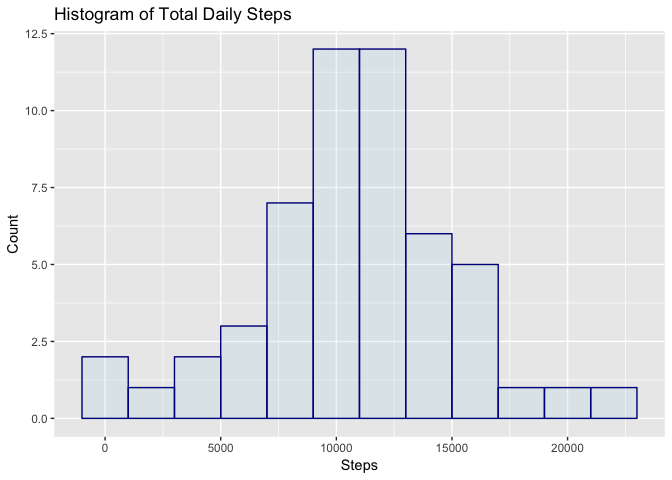
\includegraphics{PA1_template_files/figure-latex/unnamed-chunk-5-1.pdf}

\hypertarget{calculate-and-report-the-mean-and-median-of-the-total-number-of-steps-taken-per-day}{%
\subsubsection{Calculate and report the mean and median of the total
number of steps taken per
day}\label{calculate-and-report-the-mean-and-median-of-the-total-number-of-steps-taken-per-day}}

\begin{Shaded}
\begin{Highlighting}[]
\CommentTok{# calculate mean daily steps for all days}
\NormalTok{meanDailySteps <-}\StringTok{ }\KeywordTok{round}\NormalTok{(}\KeywordTok{mean}\NormalTok{(dailySteps}\OperatorTok{$}\NormalTok{dailySteps, }\DataTypeTok{na.rm =} \OtherTok{TRUE}\NormalTok{))}
\NormalTok{meanDailySteps}
\end{Highlighting}
\end{Shaded}

\begin{verbatim}
## [1] 10766
\end{verbatim}

\textbf{NOTE:} Mean daily steps are 10,766

\begin{Shaded}
\begin{Highlighting}[]
\CommentTok{# calculate median daily steps}
\NormalTok{medianDailySteps <-}\StringTok{ }\KeywordTok{round}\NormalTok{(}\KeywordTok{median}\NormalTok{(dailySteps}\OperatorTok{$}\NormalTok{dailySteps, }\DataTypeTok{na.rm =} \OtherTok{TRUE}\NormalTok{))}
\NormalTok{medianDailySteps}
\end{Highlighting}
\end{Shaded}

\begin{verbatim}
## [1] 10765
\end{verbatim}

\textbf{NOTE:} Meedian daily steps are 10,765

\hypertarget{what-is-the-average-daily-activity-pattern}{%
\subsection{What is the average daily activity
pattern?}\label{what-is-the-average-daily-activity-pattern}}

\hypertarget{plot-5-minute-interval-and-average-number-of-steps-taken}{%
\subsubsection{Plot 5-minute interval and average number of steps
taken}\label{plot-5-minute-interval-and-average-number-of-steps-taken}}

Make a time series plot of the 5-minute interval (x-axis) and the
average number of steps taken, averaged across all days (y-axis)

\begin{Shaded}
\begin{Highlighting}[]
\CommentTok{# calculate average steps for every 5 minute interval during the day and save it as a new dataframe daily pattern}
\NormalTok{dailyPattern <-}\StringTok{ }\NormalTok{data }\OperatorTok\StringTok{ }\KeywordTok{group_by}\NormalTok{(interval) }\OperatorTok\StringTok{ }\KeywordTok{summarize}\NormalTok{(}\DataTypeTok{meanActivity =} \KeywordTok{mean}\NormalTok{(steps, }\DataTypeTok{na.rm =} \OtherTok{TRUE}\NormalTok{))}

\CommentTok{# plot average 5-minute activity trend using ggplot}
\KeywordTok{ggplot}\NormalTok{(dailyPattern, }\KeywordTok{aes}\NormalTok{(interval, meanActivity)) }\OperatorTok{+}\StringTok{ }\KeywordTok{geom_line}\NormalTok{()}
\end{Highlighting}
\end{Shaded}

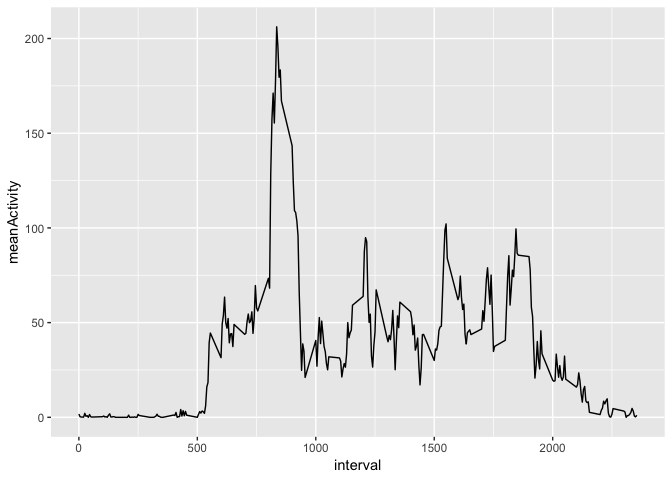
\includegraphics{PA1_template_files/figure-latex/unnamed-chunk-8-1.pdf}

\hypertarget{which-5-minute-interval-had-maximum-steps}{%
\subsubsection{Which 5-minute interval had maximum
steps?}\label{which-5-minute-interval-had-maximum-steps}}

Which 5-minute interval, on average across all the days in the dataset,
contains the maximum number of steps?

\begin{Shaded}
\begin{Highlighting}[]
\NormalTok{maxStepsInterval <-}\StringTok{ }\NormalTok{dailyPattern[}\KeywordTok{which.max}\NormalTok{(dailyPattern}\OperatorTok{$}\NormalTok{meanActivity),]}
\NormalTok{maxStepsInterval}
\end{Highlighting}
\end{Shaded}

\begin{verbatim}
## # A tibble: 1 x 2
##   interval meanActivity
##      <int>        <dbl>
## 1      835         206.
\end{verbatim}

Interval \textbf{835} had maximum average steps of \textbf{206}

\hypertarget{imputing-missing-values}{%
\subsection{Imputing missing values}\label{imputing-missing-values}}

\hypertarget{total-missing-values}{%
\subsubsection{Total Missing Values}\label{total-missing-values}}

Calculate and report the total number of missing values in the dataset
(i.e.~the total number of rows with NAs)

\begin{Shaded}
\begin{Highlighting}[]
\NormalTok{totalMissingValues <-}\StringTok{ }\KeywordTok{sum}\NormalTok{(}\KeywordTok{is.na}\NormalTok{(data}\OperatorTok{$}\NormalTok{steps))}
\NormalTok{totalMissingValues}
\end{Highlighting}
\end{Shaded}

\begin{verbatim}
## [1] 2304
\end{verbatim}

There are total 2304 number of total missing values

\hypertarget{stragety-to-fill-missing-values}{%
\subsubsection{Stragety to fill missing
values}\label{stragety-to-fill-missing-values}}

Devise a strategy for filling in all of the missing values in the
dataset. The strategy does not need to be sophisticated. For example,
you could use the mean/median for that day, or the mean for that
5-minute interval, etc.

\textbf{There is a fluctuation of activity based on the time of the day.
Hence, for each missing value we can use average for same slot across
all available values}

\hypertarget{fill-missing-values}{%
\subsubsection{Fill missing Values}\label{fill-missing-values}}

Create a new dataset that is equal to the original dataset but with the
missing data filled in.

\begin{Shaded}
\begin{Highlighting}[]
\NormalTok{newData <-}\StringTok{ }\NormalTok{data }\OperatorTok\StringTok{ }
\StringTok{             }\KeywordTok{group_by}\NormalTok{(interval) }\OperatorTok\StringTok{ }
\StringTok{             }\KeywordTok{mutate}\NormalTok{(}\DataTypeTok{steps=} \KeywordTok{ifelse}\NormalTok{(}\KeywordTok{is.na}\NormalTok{(steps), }\KeywordTok{mean}\NormalTok{(steps, }\DataTypeTok{na.rm=}\OtherTok{TRUE}\NormalTok{), steps))}

\CommentTok{# check for missing values in new DataFrame}
\KeywordTok{sum}\NormalTok{(}\KeywordTok{is.na}\NormalTok{(newData}\OperatorTok{$}\NormalTok{steps))}
\end{Highlighting}
\end{Shaded}

\begin{verbatim}
## [1] 0
\end{verbatim}

\hypertarget{histogram-of-total-steps-each-day-calculate-mean-and-median}{%
\subsubsection{Histogram of total steps each day, calculate mean and
median}\label{histogram-of-total-steps-each-day-calculate-mean-and-median}}

Make a histogram of the total number of steps taken each day and
Calculate and report the mean and median total number of steps taken per
day. Do these values differ from the estimates from the first part of
the assignment? What is the impact of imputing missing data on the
estimates of the total daily number of steps?

\begin{Shaded}
\begin{Highlighting}[]
\CommentTok{# calculate total steps by each day}
\NormalTok{dailyStepsRevised <-}\StringTok{ }\NormalTok{newData }\OperatorTok\StringTok{ }\KeywordTok{group_by}\NormalTok{(date) }\OperatorTok\StringTok{ }\KeywordTok{summarize}\NormalTok{(}\DataTypeTok{dailySteps=}\KeywordTok{sum}\NormalTok{(steps))}
\end{Highlighting}
\end{Shaded}

\begin{Shaded}
\begin{Highlighting}[]
\CommentTok{# generate histogram plot}
\KeywordTok{ggplot}\NormalTok{(dailyStepsRevised, }\KeywordTok{aes}\NormalTok{(dailySteps)) }\OperatorTok{+}\StringTok{ }
\StringTok{    }\KeywordTok{geom_histogram}\NormalTok{(}\DataTypeTok{binwidth =} \DecValTok{2000}\NormalTok{,}
                    \DataTypeTok{col=}\StringTok{"darkblue"}\NormalTok{, }
                    \DataTypeTok{fill=}\StringTok{"lightblue"}\NormalTok{, }
                    \DataTypeTok{alpha =} \FloatTok{.2}
\NormalTok{                   ) }\OperatorTok{+}\StringTok{ }
\StringTok{    }\KeywordTok{labs}\NormalTok{(}\DataTypeTok{title=}\StringTok{"Histogram of Total Daily Steps"}\NormalTok{) }\OperatorTok{+}
\StringTok{    }\KeywordTok{labs}\NormalTok{(}\DataTypeTok{x=}\StringTok{"Steps"}\NormalTok{, }\DataTypeTok{y=}\StringTok{"Count"}\NormalTok{)}
\end{Highlighting}
\end{Shaded}

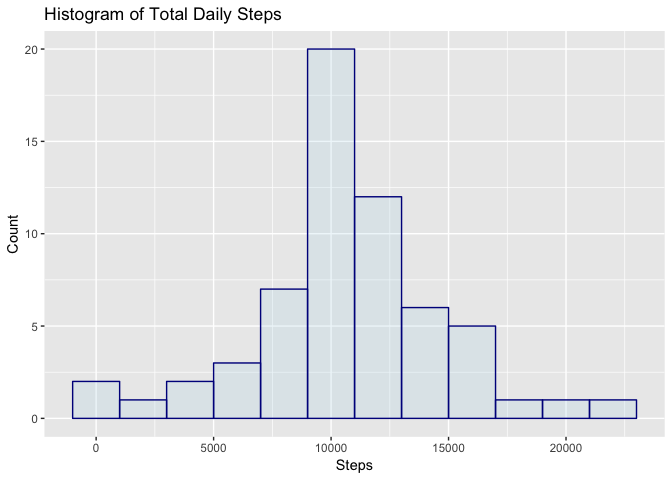
\includegraphics{PA1_template_files/figure-latex/unnamed-chunk-13-1.pdf}

\begin{Shaded}
\begin{Highlighting}[]
\CommentTok{# calculate mean daily steps for all days}
\NormalTok{meanDailyStepsRevised <-}\StringTok{ }\KeywordTok{mean}\NormalTok{(dailyStepsRevised}\OperatorTok{$}\NormalTok{dailySteps, }\DataTypeTok{na.rm =} \OtherTok{TRUE}\NormalTok{)}
\end{Highlighting}
\end{Shaded}

\begin{itemize}
\tightlist
\item
  mean daily steps are 1.0766189\times 10\^{}\{4\}
\end{itemize}

\begin{Shaded}
\begin{Highlighting}[]
\CommentTok{# calculate median daily steps}
\NormalTok{medianDailyStepsRevised <-}\StringTok{ }\KeywordTok{median}\NormalTok{(dailyStepsRevised}\OperatorTok{$}\NormalTok{dailySteps, }\DataTypeTok{na.rm =} \OtherTok{TRUE}\NormalTok{)}
\end{Highlighting}
\end{Shaded}

\begin{itemize}
\tightlist
\item
  median daily step are 1.0766189\times 10\^{}\{4\}
\end{itemize}

\hypertarget{are-there-differences-in-activity-patterns-between-weekdays-and-weekends}{%
\subsection{Are there differences in activity patterns between weekdays
and
weekends?}\label{are-there-differences-in-activity-patterns-between-weekdays-and-weekends}}

For this part the weekdays() function may be of some help here. Use the
dataset with the filled-in missing values for this part.

Create a new factor variable in the dataset with two levels --
``weekday'' and ``weekend'' indicating whether a given date is a weekday
or weekend day.

Make a panel plot containing a time series plot (i.e.~type = ``l'') of
the 5-minute interval (x-axis) and the average number of steps taken,
averaged across all weekday days or weekend days (y-axis). See the
README file in the GitHub repository to see an example of what this plot
should look like using simulated data.

\begin{Shaded}
\begin{Highlighting}[]
\NormalTok{newData}\OperatorTok{$}\NormalTok{dayOfWeek =}\StringTok{ "weekday"}
\NormalTok{newData[(}\KeywordTok{weekdays}\NormalTok{(newData}\OperatorTok{$}\NormalTok{date) }\OperatorTok\StringTok{ }\KeywordTok{c}\NormalTok{(}\StringTok{"Sunday"}\NormalTok{, }\StringTok{"Saturday"}\NormalTok{)),]}\OperatorTok{$}\NormalTok{dayOfWeek =}\StringTok{ "weekend"}
\NormalTok{newData}\OperatorTok{$}\NormalTok{dayOfWeek <-}\StringTok{ }\KeywordTok{as.factor}\NormalTok{(newData}\OperatorTok{$}\NormalTok{dayOfWeek)}
\KeywordTok{table}\NormalTok{(newData}\OperatorTok{$}\NormalTok{dayOfWeek)}
\end{Highlighting}
\end{Shaded}

\begin{verbatim}
## 
## weekday weekend 
##   12960    4608
\end{verbatim}

\begin{Shaded}
\begin{Highlighting}[]
\NormalTok{weeklyData <-}\StringTok{ }\NormalTok{newData }\OperatorTok\StringTok{ }\KeywordTok{group_by}\NormalTok{(dayOfWeek, interval) }\OperatorTok\StringTok{ }\KeywordTok{summarize}\NormalTok{(}\DataTypeTok{meanActivity =} \KeywordTok{mean}\NormalTok{(steps, }\DataTypeTok{na.rm =} \OtherTok{TRUE}\NormalTok{))}
\end{Highlighting}
\end{Shaded}

\begin{Shaded}
\begin{Highlighting}[]
\KeywordTok{ggplot}\NormalTok{(weeklyData, }\KeywordTok{aes}\NormalTok{(interval, meanActivity)) }\OperatorTok{+}\StringTok{ }
\StringTok{    }\KeywordTok{geom_line}\NormalTok{() }\OperatorTok{+}\StringTok{ }
\StringTok{    }\KeywordTok{facet_wrap}\NormalTok{(}\OperatorTok{~}\NormalTok{dayOfWeek, }\DataTypeTok{ncol=}\DecValTok{1}\NormalTok{)}
\end{Highlighting}
\end{Shaded}

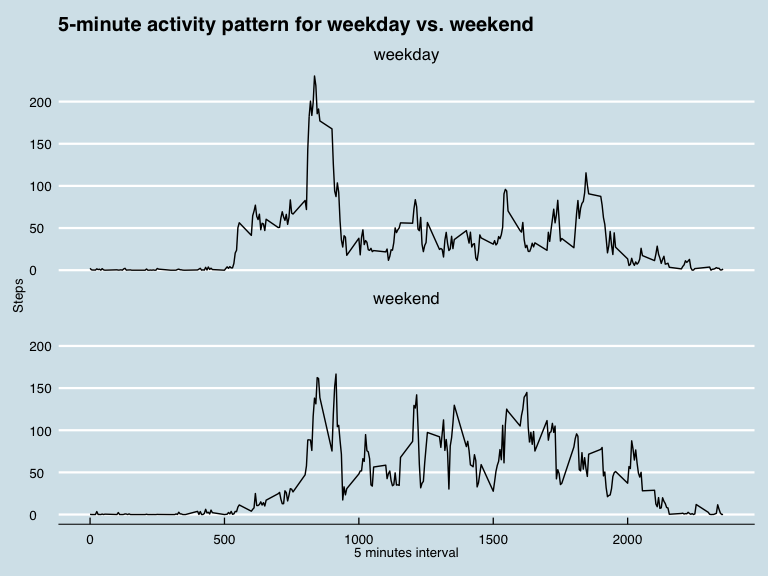
\includegraphics{PA1_template_files/figure-latex/unnamed-chunk-18-1.pdf}


\end{document}
